\chapter{CHAPTER TITLE} \label{c6}
\section{Figure}
\begin{itemize}
	\item All Figure Caption should be in the Sentence Case, TNR 10 pt, and it should be of the Format: Fig Chapter Number.Figure Number Figure Caption
	
	\item It should be cited as Fig. \ref{c6:fig1} 
	Caption must appear below the Figure.

	
	\item For Smaller: (4 Figures arranged in Two Columns) / Page; Portrait Mode.
	
	\item For Medium: (2 Figures arranged one below the other / Page; Portrait Mode.
	
	\item For Larger: 1 Figure / Page; Landscape Mode.
	
	\item Figure Label should be in Font TNR 10 pt, Bold.
	
	\item Figure Resolution should be minimum of 300 DPI.
   
    \item If the sentence starts by citing a figure, then it should be written as Figure \ref{c6:fig1}. For example, Figure \ref{c6:fig1} shows a sample picture of universe.



\end{itemize}

For example, The universe is immense and it seems to be homogeneous, 
in a large scale, everywhere we look at.

	\begin{figure}[htb]
		\begin{center}
		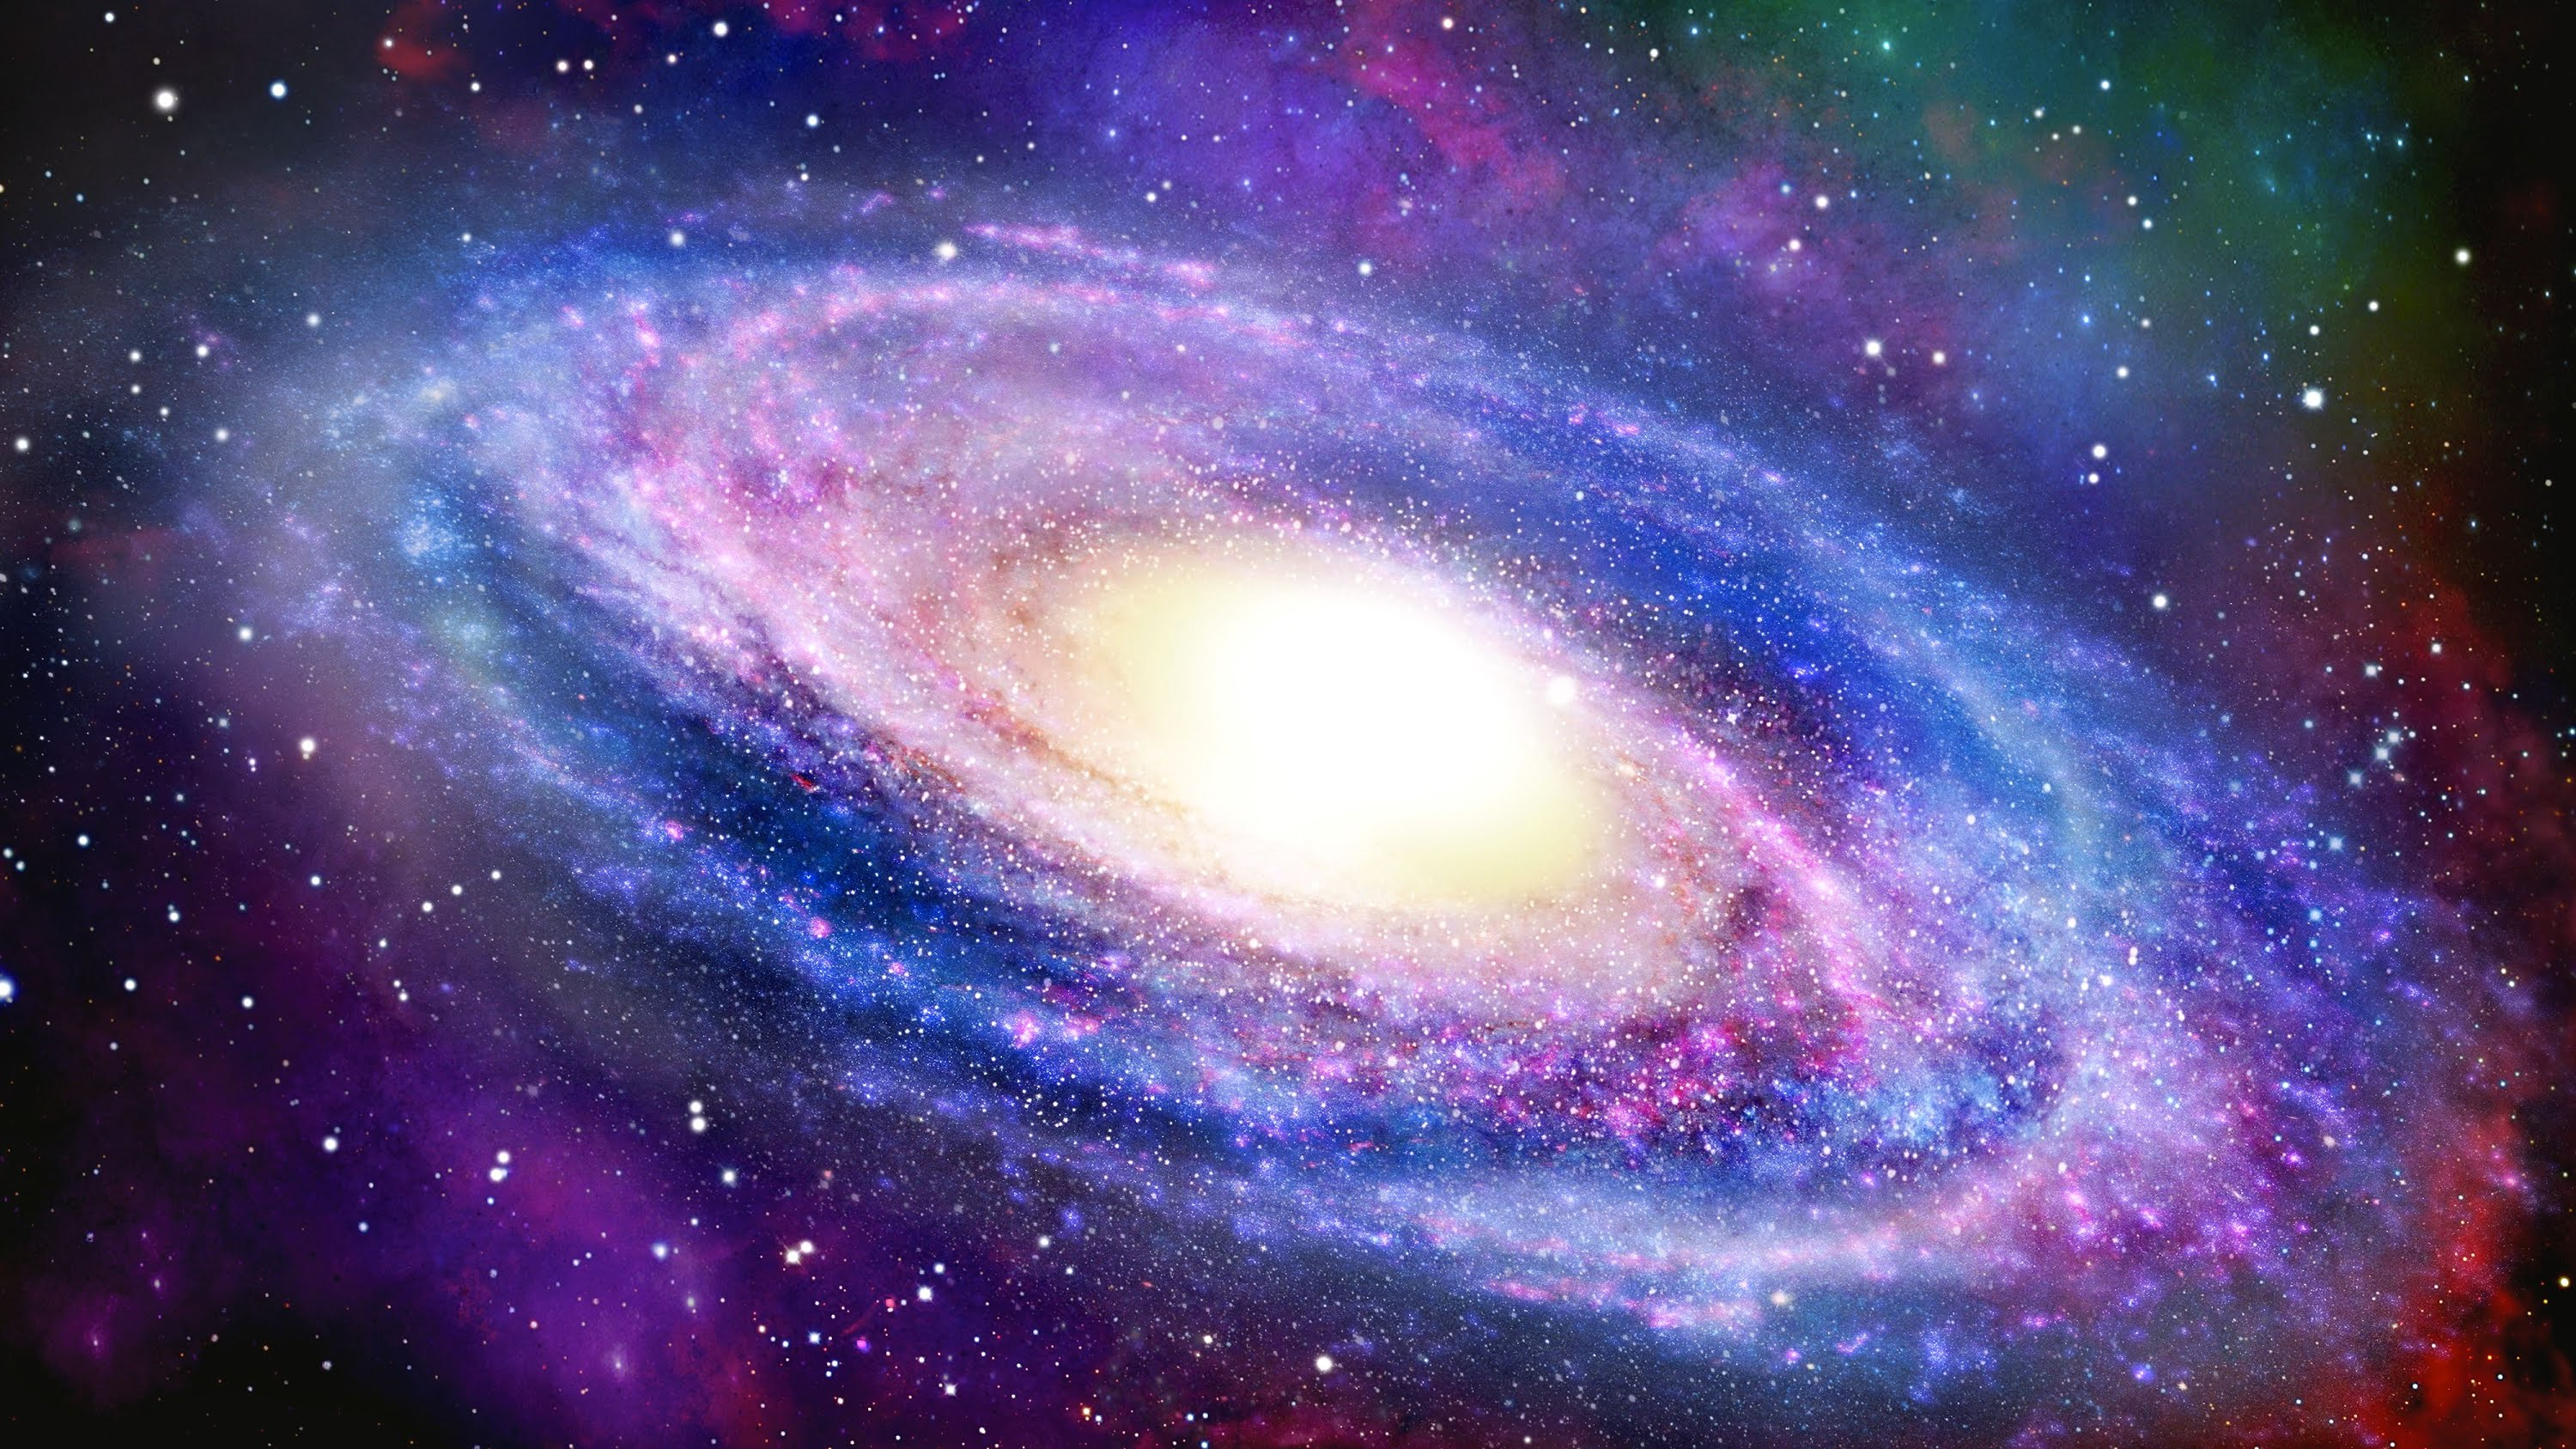
\includegraphics[scale=0.1]{universe}
	
		\caption{Sample picture of universe }
		\label{c6:fig1}
	\end{center}
	\end{figure}

There's a picture of a galaxy in Fig. \ref{c6:fig1}

\section{Graph}
Another example is given in Fig. \ref{c6:fig2}

	\begin{figure}[htb]
		\begin{center}
		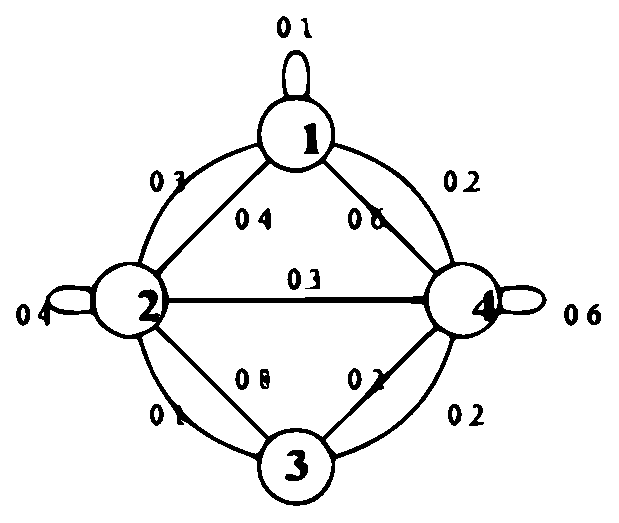
\includegraphics[scale=0.5]{graph}
	
		\caption{Sample graph }
		\label{c6:fig2}
	\end{center}
	\end{figure}

